
\mojesekce{Open source GIS-based implementation}

\justifying
{\rmfamily The SMODERP2D model belongs to a family of so called
GIS-based hydrological models utilizing capabilities of GIS software
for geodata preprocessing. This part is performed by so-called {\em
GIS providers}. Currently there are two GIS providers implemented.

\begin{itemize}
\item originally only proprietary Esri ArcGIS platform (\url{http://desktop.arcgis.com}) supported
\item new generation comes with a provider suited for open source GRASS GIS platform 
\end{itemize}
}

\subsection{GRASS GIS}
\begin{block}{GRASS GIS}
\begin{columns}
    \begin{column}{0.5\textwidth}
    \centering
    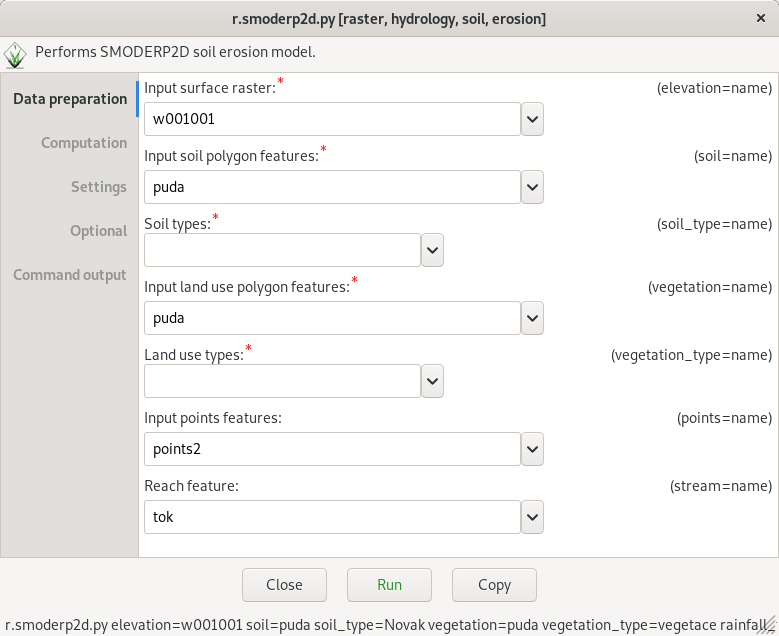
\includegraphics[width = .9\textwidth]{obr/grass.png}
    \end{column}
    \begin{column}{0.5\textwidth}
    
\includegraphics[width = .07\textwidth]{obr/grass-logo.png}
    \justifying
    {\rmfamily {\small
    {\em GRASS} (Geographic Resources Analysis Support System) {\em
    GIS} is a free and open source GIS software suite used for
    geospatial data management and analysis, image processing, spatial
    modeling, and visualization. \newline (\url{http://grass.osgeo.org})}

    \vskip 0.5em

    \begin{itemize}

    \item GRASS-based GIS provider for data preprocessing integrated
    into SMODERP2D codebase
    
    \item {\tt r.smoderp2d} GRASS Addons module for performing
    model computation including data preprocessing

    \end{itemize}
    }
    \end{column}
\end{columns}
\end{block}
\subsection{QGIS}
\begin{block}{QGIS}
\begin{columns}
    \begin{column}{0.5\textwidth}
    
\includegraphics[width = .07\textwidth]{obr/qgis-logo.png}    
    \justifying
    {\rmfamily {\small
    QGIS is a widely known free and open source cross-platform desktop
    geographic information system (GIS) application.}

    \vskip 0.5em

    \begin{itemize}
    
    \item A new QGIS plugin brings the model into QGIS environment
    while data preprocessing part is performed by integrated
    GRASS-based GIS provider
    
    \item QGIS plugin significantly increases accessibility of the
    SMODERP2D model for research purposes and also for engineering
    practice

    \end{itemize}
    
    }

    \end{column}
    \begin{column}{0.5\textwidth}
    \centering
    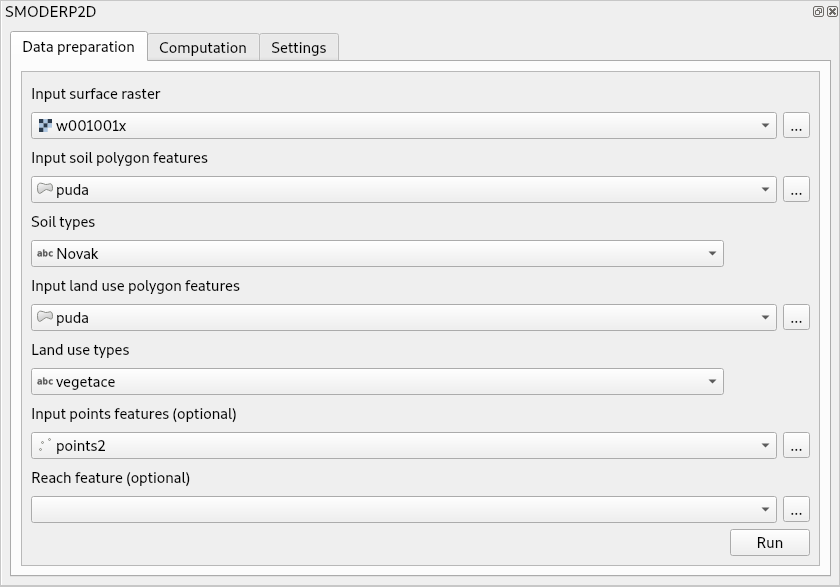
\includegraphics[width = .9\textwidth]{obr/qgis.png}
    \end{column}
\end{columns}
\end{block}

\mojesekce{Conclusions \& Results}

\justifying
{\rmfamily
% 
Conc
\begin{itemize}
    \item item1
    \item New generation of SMODERP2D model comes with Esri and GRASS-based GIS providers
    \item Accessible via ArcToolbox, GRASS Addons or QGIS plugin
\end{itemize}

}

\mojesekce{References}
\justifying
% \small{
{\rmfamily
SMODERP2D source code is licensed under GNU
GPL (\url{https://github.com/storm-fsv-cvut/smoderp2d})
% \small{
\bibliography{lit}\vspace{0.4cm}
% }
}

\mojesekce{Acknowledgment}
\justifying
{\rmfamily
The research has been supported by the research grants SGS17/173/OHK1, TJ01000270 and QK1910029.
}



\begin{beamercolorbox}[wd=\textwidth,dp=0.25cm]{cboxb}\end{beamercolorbox}\vspace{0.5cm}


\begin{columns}
    \begin{column}{0.1\textwidth}
    \centering
    
\includegraphics[width =1\textwidth]{obr/logo_TACR_dopln_AJ.png}
    \end{column}
    \begin{column}{0.5\textwidth}
    
\includegraphics[width = 1\textwidth]{obr/LogoMZeAJ.jpg}
    \end{column}
    \begin{column}{0.4\textwidth}
    powered by
    {\tiny
    \begin{lstlisting}
       @ @ @   @       @     @ @     @ @ @     @ @ @ @  @ @ @    @ @ @
      @        @ @   @ @   @     @   @     @   @        @     @  @     @
      @        @   @   @  @       @  @      @  @        @     @  @     @
        @ @    @       @  @       @  @      @  @ @ @    @ @ @    @ @ @
            @  @       @  @       @  @      @  @        @   @    @
            @  @       @   @     @   @     @   @        @    @   @
       @ @ @   @       @     @ @     @ @ @     @ @ @ @  @     @  @

      \  \  /   / /    \   \  /   \  /    /     /        @ @ @   @ @ @
       \ _\/   /_/      \   \/     \/    /_____/        @     @  @     @
           \__/          \  /      _\___/                     @  @      @
               \____      \/      /                          @   @      @
                    \_____/______/                         @     @      @
                                 \                       @       @     @
                                  \____________________ @ @ @ @  @ @ @
    \end{lstlisting}
    }
    \end{column}
\end{columns}



